% Annual progress report — Intentional Knowledge Graphs
% Compile with pdfLaTeX (Overleaf default). Bibliography: BibTeX (natbib).
\documentclass[10pt,a4paper]{article}

% ---------- page and fonts ----------
\usepackage[a4paper,margin=20mm]{geometry}
\usepackage[T1]{fontenc}
\usepackage[utf8]{inputenc}
\usepackage{lmodern}
\usepackage{microtype}
\usepackage[compact]{titlesec}
\titlespacing*{\section}{0pt}{1.6ex plus .4ex}{0.8ex}
\titlespacing*{\subsection}{0pt}{1.2ex plus .3ex}{0.5ex}
\setlength{\textfloatsep}{8pt plus 2pt minus 2pt}\setlength{\intextsep}{7pt plus 2pt minus 2pt}\setlength{\abovecaptionskip}{4pt}\setlength{\belowcaptionskip}{2pt}

% ---------- maths, tables, lists ----------
\usepackage{amsmath,amssymb}
\usepackage{booktabs}
\usepackage{array}
\usepackage{multirow}
\usepackage{enumitem}
\setlist{nosep,leftmargin=*}
\usepackage{caption}
\captionsetup{font=small,labelfont=bf}
\usepackage{subcaption}

% ---------- figures ----------
\usepackage{graphicx}
\usepackage{xcolor}
\usepackage{tikz}
\usetikzlibrary{positioning,arrows.meta,shapes.geometric,fit,calc,backgrounds,decorations.pathreplacing}
\usepackage{pgfplots}
\pgfplotsset{compat=1.18}

% ---------- colours used in every diagram ----------
\definecolor{cEntity}{HTML}{3B6EA8}     % entity nodes: blue
\definecolor{cConnector}{HTML}{D9822B}  % connector nodes: orange
\definecolor{cDoc}{HTML}{5B8C5A}        % document / text side: green
\definecolor{cModel}{HTML}{A23B72}      % a model call: plum
\definecolor{cCode}{HTML}{4A4A4A}       % deterministic code: grey
\definecolor{cStore}{HTML}{8A7E5A}      % storage: khaki
\definecolor{cLight}{HTML}{F4F4F4}

% ---------- links and references ----------
\usepackage[numbers,sort&compress]{natbib}
\usepackage[colorlinks=true,linkcolor=cEntity,citecolor=cDoc,urlcolor=cEntity]{hyperref}

% ---------- small helpers ----------
\newcommand{\code}[1]{\texttt{#1}}
\newcommand{\termdef}[1]{\textbf{#1}}
\newcommand{\eg}{e.g.\ }
\newcommand{\ie}{i.e.\ }
% shrink a diagram only when it exceeds the text block
\newcommand{\fitwidth}[1]{\resizebox{\ifdim\width>\textwidth\textwidth\else\width\fi}{!}{#1}}
\newcommand{\fitheight}[1]{\resizebox{!}{\ifdim\height>0.86\textheight 0.86\textheight\else\height\fi}{#1}}

\title{\textbf{Intentional Knowledge Graphs}\\[2mm]
\large A knowledge graph of financial quantities and the equations that relate them,\\
used as a prior for answering quantitative questions over financial documents\\[4mm]
\normalsize Annual progress report}
\author{Aditya Pugalia}
\date{November 2026 \\[1mm] \small Period covered: May 2026 -- November 2026 \quad$\cdot$\quad Code and knowledge bases: \href{https://github.com/AdityaPugalia/Intentional-Knowledge-Graphs}{github.com/AdityaPugalia/Intentional-Knowledge-Graphs}}

\begin{document}
\maketitle

\section{The task and the problem}
\label{sec:problem}

\paragraph{The task.}
An analyst is asked ``What was Amazon's days payable outstanding in fiscal 2017?'' and does four things: she chooses the right document, she knows the formula (365 times average accounts payable over cost of goods sold), she finds each input where the filing prints it (accounts payable at two year ends on the balance sheet, cost of sales on the income statement), and she checks that the numbers she copies are the ones printed, in the unit the filing uses. The task of this project is to do the same automatically for any quantitative question over a company's filings: choose the document, decide the formula, find and verify the inputs, compute the answer, and cite every number.

\paragraph{How it is done today, and where it fails.}
The systems in use retrieve a few passages by similarity to the question and ask a language model to reason over them~\citep{lewis2020rag}. On financial documents this fails at three points, each of which we measured.

\begin{enumerate}
\item \textbf{Finding the right passage.} A 10-K is long (our 84 FinanceBench filings average 143 pages) and prints the same quantity in several places under several names and scales. On FinanceBench the same model answers 9\% of questions with no document and 85\% when handed the evidence page~\citep{islam2023financebench}, so most of the difficulty is in finding the page. We measured similarity search on 5,063 quantities whose location is known from the filings' own inline-XBRL tags: the right passage is among the first results 70\% of the time (Section~\ref{sec:results}).
\item \textbf{Trusting the numbers.} The model writes down a figure whether or not it saw it. In 300 reads where the right passage was deliberately not shown, the model still cited a figure 28\% of the time, cited a wrong value 12\% of the time, and said the quantity was absent twice. Nothing in a retrieve-and-generate system checks a cited number against the printed page.
\item \textbf{Knowing the formula and the inputs.} Most quantities an analyst asks for (ratios, margins, turnover, growth) are not printed; they are computed from inputs that are scattered. Over 14,480 annual filings, only 8 accounting tags are reported by 90\% of filers; revenue alone is split over five tags (the best single one covers 39.5\% of filings, the five together 75.8\%); the inputs of a quick ratio are all printed together in 5\% of filings; the effective tax rate appears in the income-tax note of 56\% of 10-Ks and on the face of the statements almost never. The formula itself comes from the model's memory and is never stated or checked, and definitions genuinely differ: FinanceBench's own gold answers use three different quick-ratio formulas, and the authors of the best published system on it label 5 of its 150 questions ``multiple valid approaches'' and 6 ``benchmark error''.
\end{enumerate}

The three failures compound. A question that needs two inputs from two tables and a formula is answered from whichever passage ranked first, with a formula nobody sees and numbers nobody checks.

\paragraph{The claim of this project.}
Most knowledge in quantitative finance is, structurally, a system of equations over typed quantities. If that knowledge is held explicitly, as equations a solver can run, it answers the third failure directly (which formula, which inputs, whether an unprinted quantity can be reached from printed ones) and, joined to a record of where each quantity is printed, narrows the first. Section~\ref{sec:idea} gives the idea; the rest of the report shows what was built, what each measurement changed, and where it stands.

\section{The method: what makes the system}
\label{sec:idea}

\subsection{Knowledge Graphs Overview}
\label{sec:idea-pivot}



\label{sec:idea-three}
Solving Financial RAG requires 2 types of prior knowledge. (1) What different financial Concepts mean and how they are interconnected. (2) How are Financial document structured and what information do they contain. To Incorporate this we create a \emph{concept graph} which says what quantities exist and how they relate to each other, and a \emph{source graph} (Section~\ref{sec:idea-source}), which says what a document of a given kind contains. A \emph{bridge} (Section~\ref{sec:idea-bridge}),  brings them together by connecting the financial concepts to the document kinds. The edges represent the prior likelihood of each concept being found in a particular section of a document.

\begin{figure}[t]
\centering
\fitwidth{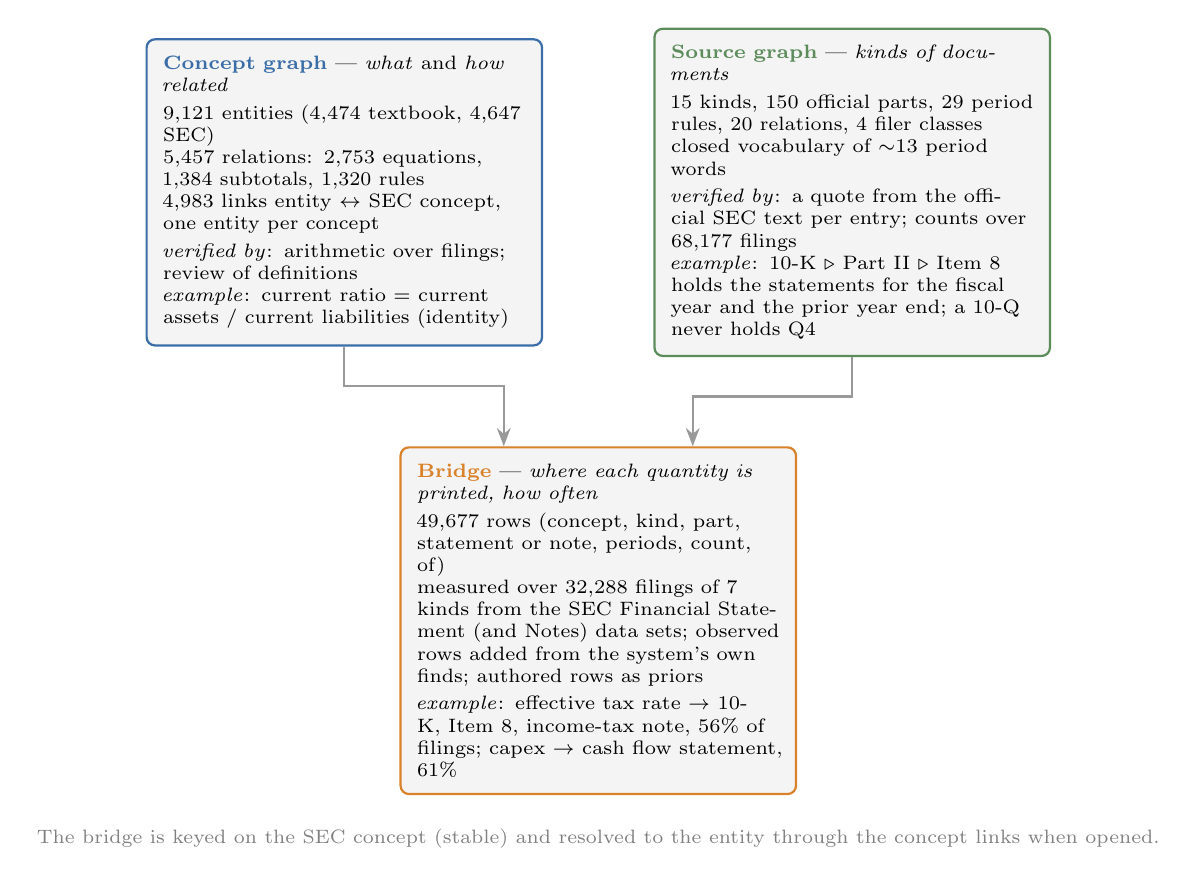
\begin{tikzpicture}[
  >=Stealth, font=\small,
  base/.style={draw,thick,rounded corners=3pt,align=left,inner sep=6pt,text width=46mm,font=\scriptsize},
  kb/.style={base,fill=cLight},
  title/.style={font=\small\bfseries},
  arr/.style={->,thick,gray!80}
]
\node[kb,draw=cEntity] (cg) at (0,0) {%
 \textcolor{cEntity}{\textbf{Concept graph}} --- \emph{what} and \emph{how related}\\[2pt]
 9{,}121 entities (4{,}474 textbook, 4{,}647 SEC)\\
 5{,}457 relations: 2{,}753 equations, 1{,}384 subtotals, 1{,}320 rules\\
 4{,}983 links entity $\leftrightarrow$ SEC concept, one entity per concept\\[2pt]
 \emph{verified by}: arithmetic over filings; review of definitions\\
 \emph{example}: current ratio $=$ current assets / current liabilities (identity)};
\node[kb,draw=cDoc,right=14mm of cg] (sg) {%
 \textcolor{cDoc}{\textbf{Source graph}} --- \emph{kinds of documents}\\[2pt]
 15 kinds, 150 official parts, 29 period rules, 20 relations, 4 filer classes\\
 closed vocabulary of $\sim$13 period words\\[2pt]
 \emph{verified by}: a quote from the official SEC text per entry; counts over 68{,}177 filings\\
 \emph{example}: 10-K $\triangleright$ Part II $\triangleright$ Item 8 holds the statements for the fiscal year and the prior year end; a 10-Q never holds Q4};
\node[kb,draw=cConnector,below=12mm of $(cg.south)!0.5!(sg.south)$] (br) {%
 \textcolor{cConnector}{\textbf{Bridge}} --- \emph{where each quantity is printed, how often}\\[2pt]
 49{,}677 rows (concept, kind, part, statement or note, periods, count, of)\\
 measured over 32{,}288 filings of 7 kinds from the SEC Financial Statement (and Notes) data sets; observed rows added from the system's own finds; authored rows as priors\\[2pt]
 \emph{example}: effective tax rate $\to$ 10-K, Item 8, income-tax note, 56\% of filings; capex $\to$ cash flow statement, 61\%};
\draw[arr] (cg.south) -- ++(0,-5mm) -| ([xshift=-12mm]br.north);
\draw[arr] (sg.south) -- ++(0,-5mm) -| ([xshift=12mm]br.north);
\node[font=\scriptsize,gray,align=center,below=3mm of br] {The bridge is keyed on the SEC concept (stable) and resolved to the entity through the concept links when opened.};
\end{tikzpicture}}
\caption{The three knowledge bases. The concept graph says what quantities exist and how they relate; the source graph says what a document of a given kind contains and for which periods; the bridge joins them by saying in which part and statement of which kind each quantity is printed, with counts. Each is verified by a different kind of evidence.}
\label{fig:three}
\end{figure}


\subsection{The Concept graph}
\label{sec:idea-graph}

The graph has two types of nodes (Figure~\ref{fig:capm}). (1) \termdef{Entity nodes} which represent financial quantities (the risk-free rate, total current assets, the effective tax rate), each with a name, aliases, type and units, a plain-language definition and a vector representation. (2) \termdef{Connector nodes} are \(n\)-ary relations which represent how different concepts interact with each other. Connector nodes can store:
\begin{enumerate}
    \item an \emph{equation} in canonical \(f(x_1,\dots,x_n)=0\) form where the inputs are the entities involved in the equation. t also stores the assumptions under which the equation holds
    \item \emph{rules} which store textual information on how different entities affect each other
    \item \emph{aggregation} (a subtotal with a signed, weighted edge per member ever observed).
\end{enumerate}
In the graph edges only connect to each other via connectors. A connector may reference both entities and other connectors. Connectors also have a trust level associated with them based on how likely the relation is to hold in real life.

\begin{figure}[t]
\centering
\fitwidth{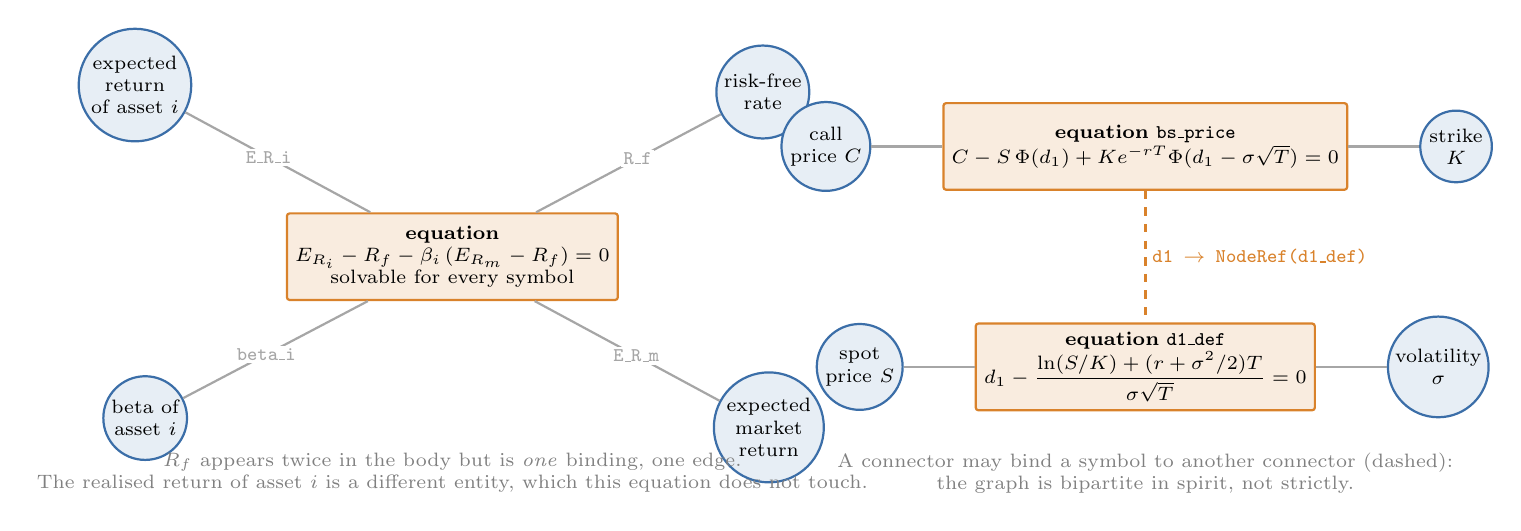
\begin{tikzpicture}[
  >=Stealth,
  ent/.style={circle,draw=cEntity,fill=cEntity!12,thick,minimum size=9mm,font=\scriptsize,align=center,inner sep=1pt},
  con/.style={rectangle,draw=cConnector,fill=cConnector!15,thick,rounded corners=1pt,minimum width=36mm,minimum height=11mm,font=\scriptsize,align=center,inner sep=3pt},
  lab/.style={font=\scriptsize\ttfamily,fill=white,inner sep=1pt},
  every edge/.style={draw,thick,gray!70}
]
% ---------- CAPM ----------
\node[con] (capm) at (0,0) {\textbf{equation} \\ $E_{R_i} - R_f - \beta_i\,(E_{R_m} - R_f) = 0$ \\ solvable for every symbol};
\node[ent,above left=11mm and 14mm of capm] (eri) {expected\\return\\of asset $i$};
\node[ent,above right=11mm and 14mm of capm] (rf) {risk-free\\rate};
\node[ent,below left=11mm and 14mm of capm] (beta) {beta of\\asset $i$};
\node[ent,below right=11mm and 14mm of capm] (erm) {expected\\market\\return};
\path (eri) edge node[lab,pos=.45]{E\_R\_i} (capm);
\path (rf) edge node[lab,pos=.45]{R\_f} (capm);
\path (beta) edge node[lab,pos=.45]{beta\_i} (capm);
\path (erm) edge node[lab,pos=.45]{E\_R\_m} (capm);
\node[font=\scriptsize,gray,align=center,below=18mm of capm] {$R_f$ appears twice in the body but is \emph{one} binding, one edge.\\ The realised return of asset $i$ is a different entity, which this equation does not touch.};

% ---------- connector referencing connector ----------
\begin{scope}[xshift=88mm]
\node[con] (d1) at (0,-14mm) {\textbf{equation} \texttt{d1\_def} \\ $d_1 - \dfrac{\ln(S/K)+(r+\sigma^2/2)T}{\sigma\sqrt T} = 0$};
\node[con] (bs) at (0,14mm) {\textbf{equation} \texttt{bs\_price} \\ $C - S\,\Phi(d_1) + K e^{-rT}\Phi(d_1-\sigma\sqrt T) = 0$};
\node[ent,left=9mm of d1] (S) {spot\\price $S$};
\node[ent,right=9mm of d1] (sig) {volatility\\$\sigma$};
\node[ent,left=9mm of bs] (C) {call\\price $C$};
\node[ent,right=9mm of bs] (K) {strike\\$K$};
\path (S) edge (d1); \path (sig) edge (d1); \path (C) edge (bs); \path (K) edge (bs);
\path (bs) edge[dashed,cConnector,very thick] node[lab,right=1pt,pos=.5]{d1 $\to$ \texttt{NodeRef(d1\_def)}} (d1);
\node[font=\scriptsize,gray,align=center,below=4mm of d1] {A connector may bind a symbol to another connector (dashed):\\ the graph is bipartite in spirit, not strictly.};
\end{scope}
\end{tikzpicture}}
\caption{The entity--connector graph. Left: CAPM as one equation connector (orange) bound to four entity nodes (blue) by undirected edges carrying the local symbol. The expected returns are entities in their own right; no edge or expression applies $E[\cdot]$. Right: a connector referencing another connector, the $d_1$ definition used inside the Black--Scholes call price. $r$ and $T$ are omitted from the drawing for space.}
\label{fig:capm}
\end{figure}



To compute a target, the \termdef{solver} searches the graph as an AND/OR tree.
A target at a coordinate (company, period, segment) is an \emph{OR-node}: it can
be produced by any one of the connectors that produce it. Each connector is an
\emph{AND-node}: it can be used only when all its other inputs are available, and
each of those inputs becomes a target in turn. The solver explores this tree by
iterative deepening and memoises failed targets so that they are not tried twice. The node expansion is done by order of trust followed by cost (the number of new inputs required to compute our target).



\subsection{The source graph}
\label{sec:idea-source}

The \termdef{source graph} is the second knowledge graph. It describes kinds of documents and their official parts. For example a 10-K has Items 1--15 and Item~8 holds the statements, etc. It includes Fifteen kinds and 150 parts based on the official SEC guidelines. Each entry has a description, a verified quote, the time periods a part holds, and its vector embedding.

\subsection{The bridge}
\label{sec:idea-bridge}

The \termdef{bridge} contains the likelihood of finding concepts in any part of a document. It says in which part, statement or note of which kind each quantity is printed and for which time periods. The likelihood is computed using 32,288 random filings from the SEC's Financial Statement and Notes data sets by counting the appearances of each concept in those filings. 

\subsection{Agent Reasoning Loop}
\label{sec:impl-loop}

Figure~\ref{fig:loop} shows the agent loop that answers a question. A language model is called at eight points in the loop, and at each point it makes one narrow choice; everything in between is done by deterministic code. The eight steps are as follows.
\begin{enumerate}[label=(\arabic*)]
  \item \textbf{Understand.} The model first reads the question on its own, before any document is opened, and extracts what is needed to answer it. It returns the targets, that is, the quantities the question asks for, named as the question names them and with their coordinates (company, period and segment). It also returns a formula over these targets, but only when the question spells one out, together with the information given in the question, the unit the answer should be expressed in, and an analysis flag when the question asks for something to be judged rather than only computed.
  \item \textbf{Map.} The words naming each target are then mapped to exactly one entity of the concept graph, or to none if no entity fits. Candidate entities are gathered in three ways: by their names, by the captions that filers print for the corresponding SEC concept, and by vector similarity search. The model is shown the candidates together with their definitions and makes the choice.
  \item \textbf{Choose documents.} The model next chooses which stored documents to read. It does so through tools over the stored document covers, over the periods that each kind of document holds according to the source graph, and over a company store of 16,416 filers and their co-registrants. A prior year that a document holds only as a comparative is ranked below the document's own year, and the tool states this. When only one document fits the question, the choice is made by code without calling the model.
  \item \textbf{Search or derive.} Code then decides whether to search for the target directly or to derive it from other quantities. The decision is based on the bridge's calibrated probability that a filing of this kind, in this industry, prints the entity. If that probability is high, the system searches for the value; if it has been measured as zero, the system tries formulas first; and if it is unknown, the system searches first and derives the value only if the search fails.
  \item \textbf{Routes.} When a target has to be derived, the system collects the relations of the concept graph that produce the entity and solves each of them symbolically for the target. These routes are ranked first by trust and then by the joint probability that all of their inputs will be found. The joint probability is counted in sequence rather than by treating the inputs as independent, because the presence of one quantity in a filing strongly predicts the presence of another: current liabilities is reported by 98.8\% of the filers that report current assets, but by only 3.9\% of the others.
  \item \textbf{Find.} The model then looks for each needed value in the chosen document. It searches first in the parts that the bridge names for that quantity, and only afterwards in the whole document. It reads whole tables together with the text chunks around them, and replies with one of six outcomes: \emph{found}, \emph{found text}, \emph{collect}, \emph{widen}, \emph{search again} or \emph{absent}.
  \item \textbf{Plan.} Code keeps the state of the search, and this state serves as the system's memory from one step to the next. When an input is found, its value is propagated up through every route that it completes. When a route fails because one of its inputs cannot be found, the cheapest of the paused routes is activated in its place.
  \item \textbf{Respond and evaluate.} Finally, every derived value is recomputed in code from its cited inputs, using the equation reloaded from the graph, so that no arithmetic is taken from the model. If the question asks only for a number, the answer is returned without any model call. Otherwise a single model call writes the answer, and every claim in it must quote the evidence it rests on. Code then corrects the shape, unit and sign of the answer.
\end{enumerate}

\begin{figure}[p]
\centering
\fitheight{\fitwidth{\begin{tikzpicture}[
  >=Stealth, font=\scriptsize, node distance=3.5mm,
  step/.style={draw,thick,rounded corners=3pt,align=center,inner sep=4pt,text width=52mm,minimum height=11mm},
  model/.style={step,draw=cModel,fill=cModel!8},
  code/.style={step,draw=cCode,fill=cLight},
  kbnote/.style={draw=cConnector,thick,rounded corners=2pt,fill=cConnector!10,align=left,inner sep=3pt,text width=48mm,font=\tiny},
  arr/.style={->,thick,gray!80},
  back/.style={->,thick,cModel,dashed}
]
\node[model] (und) at (0,0) {\textbf{1 Understand} \textcolor{cModel}{[model]}\\ targets + coordinates, formula over targets, givens, unit, analysis statement};
\node[model,below=of und] (map) {\textbf{2 Map words $\to$ entity} \textcolor{cModel}{[model]}\\ candidates by words, filer captions and meaning; a number or \emph{none}; never cached};
\node[model,below=of map] (docs) {\textbf{3 Choose documents} \textcolor{cModel}{[model, or code when one fits]}\\ tools: search documents, company filers, list};
\node[code,below=of docs] (dec) {\textbf{4 Search or derive?} [code]\\ calibrated chance from the bridge, nearest industry first:\\ high $\to$ search; measured 0 $\to$ formulas; unknown $\to$ search then derive};
\node[model,below=of dec] (routes) {\textbf{5 Routes} \textcolor{cModel}{[model when several]}\\ formulas solved for the target, ranked by trust then joint chance of inputs; ancestors excluded; a definition stated by the model when the graph has none};
\node[model,below=of routes] (find) {\textbf{6 Find} \textcolor{cModel}{[model, rounds $\le 3$]}\\ scope: the parts the bridge names; passages from the retriever; reply: found / found text / collect / widen / search / absent};
\node[code,below=of find] (ground) {\textbf{Ground} [code]\\ quote printed in the passage and row; value and sign from the cell; unit from quoted evidence; kind of number vs kind of quantity};
\node[code,below=of ground] (plan) {\textbf{7 Plan state} [code]\\ settle, propagate up complete routes; switch to a cheaper paused route; abandon inputs no longer needed; evidence kept in full};
\node[model,below=of plan] (resp) {\textbf{8 Respond} \textcolor{cModel}{[model; none for a bare number]}\\ every derived value recomputed from cited inputs via the graph's equation; claims must quote evidence; may ask for more targets};
\node[code,below=of resp] (eval) {\textbf{Evaluate} [code; model only to restate]\\ shape, unit, sign fixed; percentage points for rate differences};
\draw[arr] (und) -- (map); \draw[arr] (map) -- (docs); \draw[arr] (docs) -- (dec); \draw[arr] (dec) -- (routes);
\draw[arr] (dec.east) -- ++(6mm,0) |- node[pos=.25,right,font=\tiny,align=left]{search\\first} (find.east);
\draw[arr] (routes) -- (find); \draw[arr] (find) -- (ground); \draw[arr] (ground) -- (plan); \draw[arr] (plan) -- (resp); \draw[arr] (resp) -- (eval);
\draw[back] (ground.west) -- ++(-5mm,0) |- node[pos=.25,left,font=\tiny,align=right]{rejected:\\ re-ask once} (find.west);
\draw[back] (plan.west) -- ++(-10mm,0) |- node[pos=.3,left,font=\tiny,align=right]{input absent:\\ expand through\\ a formula, or\\ switch route} (routes.west);
\draw[back] (resp.west) -- ++(-15mm,0) |- node[pos=.3,left,font=\tiny,align=right]{needs:\\ new targets\\ ($\le 2$ rounds)} (map.west);

% knowledge-base notes on the right
\node[kbnote,right=12mm of map] (n1) {\textcolor{cEntity}{\textbf{concept graph}}: names, aliases, SEC concept links, filer captions, vectors};
\node[kbnote,right=12mm of docs] (n2) {\textcolor{cDoc}{\textbf{source graph}} + company store: which stored document covers the company and period, as its own year or a comparative};
\node[kbnote,right=12mm of dec] (n3) {\textcolor{cConnector}{\textbf{bridge}}: share of filings of this kind and industry printing the entity; in which part and statement};
\node[kbnote,right=12mm of routes] (n4) {\textcolor{cEntity}{\textbf{concept graph}}: equations and subtotals that produce the entity, solved symbolically; trust: identity $<$ law $<$ empirical};
\node[kbnote,right=12mm of find] (n5) {\textcolor{cConnector}{\textbf{bridge}} $\to$ parts to search first; \textcolor{cDoc}{\textbf{source graph}} $\to$ headings linked to parts; retriever v3 ranks chunks};
\node[kbnote,right=12mm of resp] (n6) {\textcolor{cEntity}{\textbf{concept graph}}: the equation reloaded by connector id for recomputation in code};
\foreach \a/\b in {n1/map,n2/docs,n3/dec,n4/routes,n5/find,n6/resp} {\draw[arr,gray!50] (\a.west) -- (\b.east);}
\end{tikzpicture}}}
\caption{The question-answering loop (version 4). Plum boxes are the points where a model is called, each with one narrow choice; grey boxes are code. Dashed arrows are the loop's backtracking paths. The notes on the right say which knowledge base each step consults.}
\label{fig:loop}
\end{figure}


The rule that runs through the whole loop is \textbf{grounding}. A figure enters an answer only if the code finds the model's quote printed in the cited passage and in the cited row; the value and its sign are then taken from the table cell, not from the model. A unit is accepted when the evidence quoted for it is found in the table heading or the surrounding context, and is otherwise recorded as an assumption. All arithmetic runs in code, with every value normalised to base units and checked for dimensional consistency. What the code deliberately does \emph{not} do is assume the shape of a document: identity tie-outs and range checks are not enforced. When a value disagrees with the graph, the disagreement is put to the model once, and if it remains it is recorded as a flag.

\subsection{Learned where learning is safe}
\label{sec:impl-retrieval}

A hand-ordered search was replaced by \emph{one score per chunk}: thirteen signals (words, synonym, table row label, heading path, meaning, the bridge's share for the part in force, the coordinate's words near and far, table and number counts, length) fitted as a conditional logit~\citep{mcfadden1974} with a ``not printed in this document'' alternative, so it returns a probability over chunks and a probability that the target is absent. The training data is the methodological point: 420 EDGAR filings from two SEC quarters disjoint from the bridge's five, labelled by their own inline-XBRL tags (178,185 values and 23,195 text blocks with the chunks that print them), the benchmark companies excluded, held out by company. No model call and no benchmark question supervises anything. The served probability mass and the bridge's counts were then calibrated on held-out filings~\citep{zadrozny2002}, because both under-predicted in the middle of their range. The principle is general: a piece whose behaviour can be fitted on data the system is never evaluated on is fitted; a judgement about meaning is made by a model every time; a check against the document stays hard and a check against the graph only asks.

\section{What is new against existing work}
\label{sec:novelty}

Table~\ref{tab:compare} places the system against the families of work it touches, on the four decisions of Section~\ref{sec:idea}. The literature was searched for each; the paragraphs below give the nearest precedents and the exact difference.

\begin{table}[h]
\centering\footnotesize
\caption{The four design decisions against the nearest existing work. ``Facts fixed at ingest'' means the document is turned into facts or triples once, before any question is seen.}
\label{tab:compare}
\setlength{\tabcolsep}{4pt}\begin{tabular}{@{}>{\raggedright\arraybackslash}p{33mm}>{\raggedright\arraybackslash}p{27mm}>{\raggedright\arraybackslash}p{25mm}>{\raggedright\arraybackslash}p{16mm}>{\raggedright\arraybackslash}p{23mm}>{\raggedright\arraybackslash}p{30mm}@{}}
\toprule
 & relations are & formula comes from & facts fixed at ingest & cited number checked in code & where-to-look knowledge \\
\midrule
GraphRAG, LightRAG, financial KG-RAG~\citep{edge2024graphrag,guo2024lightrag,shah2024multidoc,arun2025finreflectkg} & binary triples written by a model & the model & yes & no & none \\
FIBO; XBRL calculation linkbase~\citep{bennett2013fibo,xbrl2003spec} & classes and properties; signed sums within one context & --- & --- & --- & none \\
Program-of-thought QA: FinQA line, TAT-LLM, FINDER~\citep{chen2021finqa,khatuya2025finder} & --- & the model writes the program & gold table given & executed, not checked against the page & none \\
Formula retrieval: FinanceReasoning~\citep{tang2025financereasoning}; VeriFin~\citep{hall2026verifin} & Python functions by similarity; a provenance order over sources & retrieved; VeriFin verifies another system's answer with Z3 over XBRL facts & --- & VeriFin: yes, against XBRL facts & none \\
Structure-aware retrieval: PageIndex, HC-RAG, FinGEAR, HiREC~\citep{vectify2026mafin,chen2026hcrag,li2025fingear,choe2025hirec} & --- & the model & no & no & the Item hierarchy as a lexicon or tree, not measured \\
\midrule
\textbf{this project} & \(n\)-ary equation nodes, canonical \(f=0\), solvable for any variable; admitted only when filings confirm them & the graph; a model's definition only when the graph has none, recorded as an assumption & no: text and tables stored whole & yes: quote, row, sign and unit words, before use & measured over 32,288 filings; decides search vs derive and where to start \\
\bottomrule
\end{tabular}
\end{table}

\paragraph{Relations as solvable nodes.}
Graph-based retrieval systems, GraphRAG and LightRAG and the financial knowledge graphs built on 10-Ks and news~\citep{edge2024graphrag,guo2024lightrag,shah2024multidoc,arun2025finreflectkg}, extract binary triples with a model at index time and hand them to the generator as context; the surveys of the field describe no design in which a node owns an executable body. On filings they do not help much: FinSage measured GraphRAG at 42.5\% and LightRAG at 13.7\% on its filings questions against its own 82.7\%~\citep{wang2025finsage}. The financial ontologies hold classes and properties with no arithmetic~\citep{bennett2013fibo}; the XBRL calculation linkbase holds signed sums within one reporting context, no ratios and no roll-forwards~\citep{xbrl2003spec}, and we use its 6,514 arcs only as candidates that must still be observed to hold. Hoffman's impute rules~\citep{hoffman2017theory} derive an unreported fact from reported ones, but are hand-authored, directional and tied to a reporting style. The closest design to our equation node is Wolfram's \code{FormulaData}~\citep{wolfram_formuladata}, a curated library of named formulas solvable for any variable; it is fixed, has no finance coverage and no admission test against data. We found no prior graph whose relations are \(n\)-ary equations admitted by measurement over filings.

\paragraph{The formula from a verified graph, not the model.}
The program-of-thought line that dominates numerical financial QA (FinQA, TAT-QA, ELASTIC, APOLLO, FINDER, TAT-LLM; best FinQA execution accuracy 75.3\% against 92.3\% human~\citep{chen2021finqa,khatuya2025finder}) has the model write the program, executes it, and never looks the formula up or checks it; the datasets also hand over the one gold table. Two 2025--26 works move the formula out of the model. FinanceReasoning retrieves the three nearest of 3,133 Python functions by embedding similarity and finds that this beats passage retrieval (GPT-4o 83.2 to 91.6\%)~\citep{tang2025financereasoning}, but the functions are unverified snippets and there is no document, no citation check and no prior on where a quantity is printed. VeriFin~\citep{hall2026verifin} is a verifier rather than an answerer: it grounds operands in XBRL facts, checks another system's answer with an SMT solver and abstains otherwise, under a strict order of formula authority in which a model is never a source; on a 67-question numeric subset of FinanceBench it accepts 70\% of answers at 86.7\% accuracy. It therefore covers only XBRL-tagged quantities and works after the fact. Our graph admits a formula by filing-wide statistical verification rather than by provenance class, produces the answer from the document text, and chooses between searching and deriving from measured chances.

\paragraph{Read at question time, checked in code.}
Every knowledge-graph system above commits to its facts at ingest, which is the failure Table~\ref{tab:commitment} measures. Grounding work in finance adds a traceability layer to a production assistant~\citep{kabra2026verifiable} or benchmarks claim verification over long documents; none checks, before a number is used, that the model's quote is printed in the cited passage and row and takes value, sign and unit from the page rather than from the model. PageIndex~\citep{vectify2026mafin}, the strongest published FinanceBench system, shares one idea with us, an index built from the document's own layout for a model to reason over, and none of the other three: its formula is the model's, nothing is recomputed and no citation is checked.

\paragraph{Where to look, measured; learned pieces trained on filings' own labels.}
Item-level routing of 10-K questions exists as a lexicon (FinGEAR~\citep{li2025fingear}), a document-then-passage hierarchy (HiREC~\citep{choe2025hirec}) or a typed evidence tree (HC-RAG~\citep{chen2026hcrag}); none estimates from data the probability that a given quantity is printed in a given part of a given kind of filing, and none uses it to decide whether to search or to derive. Inline XBRL has been used as free supervision for tagging numbers with concepts (FiNER~\citep{loukas2022finer}), not for training a retriever; we found no retriever fitted on filings' own tags, company-disjoint from every evaluation document.

\section{Results}
\label{sec:results}

Every design change in this report was made after a measurement, and most of the measurements were made on real filings with no model call. This section reports the ones that matter for judging the state of the work: the solver on textbook questions, the verification of the SEC relations, the retrieval and reading measurements on held-out filings, and three full runs over FinanceBench.

\subsection{The solver on textbook questions}

A benchmark of 32 end-of-chapter problems from a corporate-finance textbook (CAPM, Gordon growth, WACC, DuPont, bond pricing, Hamada, break-even) was built with gold answers computed in code. Each problem carries the book's wording and an \emph{oracle} form in the graph's own entity names, so that the solver can be measured apart from the naming problem. Table~\ref{tab:textbook} shows the progression.

\begin{table}[h]
\centering\small
\caption{The 32-question textbook benchmark, solver only, no model calls. The oracle rows measure the graph and solver with naming taken out; the first two rows measure the whole gap.}
\label{tab:textbook}
\begin{tabular}{llr>{\raggedright\arraybackslash}p{72mm}}
\toprule
when & naming & correct & note \\
\midrule
Aug 2026 & the book's wording, exact match & 1/32 & no fuzzy resolution in front of the solver \\
Aug 2026 & the book's wording, token overlap & 1/32 & name coverage 8 $\to$ 25 of 32, nothing more solved: linking to \emph{an} entity is useless unless it is the one the equation binds \\
Aug 2026 & the graph's own names & 16/19 & all three failures are CAPM: $E[\cdot]$ as an inert function cannot be inverted; 3 time-outs at 25 s \\
Aug 2026 & same, new solver & 16/19 & 0 time-outs, solved items $\le 0.3$ s; CAPM gives up at the budget \\
Sep 2026 & same, statistics as entities & \textbf{19/19} & CAPM solves in $\le 1$ s; the whole run 7 s instead of 48 s \\
Oct 2026 & same, after repairs and merges & \textbf{19/19} & three probes renamed to the corrected entities \\
\bottomrule
\end{tabular}
\end{table}

Two lessons were general. First, the substrate was sound from the start: every law probed was present and correctly formed and solved instantly once addressed by its name. Second, the naming gap is a \emph{disambiguation} problem, not a threshold problem: of 76 oracle names probed, only 5 had a single candidate entity (``present value'' competed with 21). That finding is what later made ``map words to one entity, by a model shown the definitions, every time'' the rule, and what motivated the entity repairs and merges of October.

\subsection{Relations verified against filings}

Table~\ref{tab:verify} gives the admission rates of representative relations in the SEC concept graph. The numbers are the fraction of annual filings reporting all operands on which the relation holds within 0.5\%. They are reported here because they are the evidence that the graph's relations are true of real documents and not only of textbooks, and because the refusals are as informative as the admissions.

\begin{table}[h]
\centering\small
\caption{Verification of relations against the SEC numeric data (five quarters, 4.6M consolidated values). A relation below 0.5 is refused, 0.5--0.7 admitted as empirical, above as identity.}
\label{tab:verify}
\begin{tabular}{>{\raggedright\arraybackslash}p{88mm}lr}
\toprule
relation & kind & holds in \\
\midrule
assets $=$ liabilities $+$ equity & identity & 99.9\% \\
cash reconciliation (beginning $+$ change $=$ ending) & identity & 99\% \\
gross profit $=$ revenue $-$ cost of revenue & identity & 98.6\% \\
cash roll-forward through the cash-flow statement & identity & 98\% \\
current ratio $=$ current assets / current liabilities & identity (definition) & solves out of the box \\
subtotals (assets, liabilities, current assets, equity, investing and financing cash flow) & aggregation & 91--97\% of filings explained \\
working-capital roll-forwards through cash-flow lines & empirical & 35--60\% \\
IFRS operating-cash-flow reconciliation & aggregation & 72\% (US GAAP: 37\%) \\
pre-tax income $=$ operating income $-$ interest expense $+$ other & \emph{refused} & 36\% \\
treasury-stock roll-forwards & \emph{dropped} & $\approx 50\%$ (half of filers reissue) \\
\bottomrule
\end{tabular}
\end{table}

\subsection{The graph as a store: the measured failure}

The graph-as-store path was run twice end to end on a real combined 10-K from DocFinQA~\citep{reddy2024docfinqa} and answered 0 of 11 questions both times; its per-decision accuracies are in Table~\ref{tab:commitment}. A hand audit of 25 random extracted facts against their source rows found 9 wrong before fixes and 6 after, and an automated pass over 9,433 facts flagged 18\% with a verified fact-to-row mapping; the best estimate was that about one fact in four carried at least one wrong label. The model-based table reader that replaced the code reader improved every coordinate (facts with no period 46\% $\to$ 19\%, with no company 52\% $\to$ 16\%) and still answered nothing, because 31\% of linked cells held more than one distinct value and the question that would have told them apart was not available at ingest. This is the measurement behind the change of direction.

\subsection{Retrieval on held-out filings}

Table~\ref{tab:retrieval} reports the learned retriever on 5,063 needs from companies never used in the fit, with the hand-ordered ladder on the same needs. The right chunk is known from the filing's own inline-XBRL tags; no benchmark question is involved.

\begin{table}[h]
\centering\small
\caption{Retrieval on 5,063 held-out needs (3,985 printed, 1,078 not printed) from 2025 EDGAR filings of companies excluded from training. Recall@$k$: the labelled chunk is among the first $k$ served.}
\label{tab:retrieval}
\begin{tabular}{lrrrrr}
\toprule
 & recall@1 & recall@5 & recall@9 & MRR & ``not printed'' AUC \\
\midrule
learned scorer (v3), all signals & \textbf{0.596} & \textbf{0.882} & \textbf{0.927} & \textbf{0.721} & 0.817 \\
\quad numeric needs (3,062) & & 0.912 & & & \\
\quad text needs (923) & & 0.780 & & & \\
\quad without words & 0.354 & 0.732 & & 0.518 & 0.666 \\
\quad without meaning & 0.581 & 0.857 & & 0.702 & 0.794 \\
\quad without place (bridge, part tag) & 0.589 & 0.876 & & 0.714 & 0.818 \\
\quad words only & 0.535 & 0.806 & & 0.654 & 0.801 \\
\midrule
ladder (v2), first call (mean 6.4 passages) & & 0.704 & & & \\
ladder (v2), with a second call & & 0.774 & & & \\
\bottomrule
\end{tabular}
\end{table}

The ablations say where the gain comes from: the words are indispensable, the meaning vector adds 2.5 points of recall@5 and the count of numbers printed is the largest single weight, while the bridge's share is statistically significant but small, because it rarely separates chunks \emph{within} one document (its value is in deciding whether to search at all and where to start). Calibration of the served probability mass against hit rate reduced the log loss from 0.446 to 0.429 on the check half and brought every bin within four points.

\subsection{The reader}

The remaining number the loop needs is how often the model, shown the right chunk, cites the right cell. Five hundred single reads were run with the finder's own prompt over held-out needs (Table~\ref{tab:reader}). The misses on numbers are mostly the model asking for another period or a total the shown tables do not have; ``absent'' is almost never said (2 of 300); the rejections are almost all a dash cell cited as zero, which the grounding refuses. When the target was \emph{not} served the model nonetheless cited something 28\% of the time, a wrong value 12\% of the time, which is the rate at which a find against a low retrieval chance must be doubted.

\begin{table}[h]
\centering\small
\caption{Single reads with the finder's prompt, 500 needs of held-out companies, 10-K rows (10-Q rows were affected by a harness error in the coordinate and are not reported).}
\label{tab:reader}
\begin{tabular}{llrrrrr}
\toprule
stratum & kind & $n$ & cited right & right value anywhere & missed & cited a wrong value \\
\midrule
number, right chunk served & 10-K & 134 & 69\% & 79\% & 10\% & 1\% \\
text, right chunk served & 10-K & 44 & 75\% & 75\% & 25\% & 0\% \\
number, right chunk not served & 10-K & 43 & 7\% & 23\% & 56\% & 12\% \\
\bottomrule
\end{tabular}
\end{table}

\subsection{FinanceBench, three full runs}

FinanceBench~\citep{islam2023financebench} has 150 questions over 84 SEC filings and earnings releases (10-K, 10-Q, 8-K, releases; 12,013 pages), every question naming its company and period, with an evidence page and a gold answer. All 84 documents were parsed and ingested (84 heading outlines, 1,673 headings linked to parts). The system is given the question only; it chooses the document. 52 gold answers are a bare number and are scored in code (within tolerance, or rounding to the gold at the decimals it prints); the other 98 are sentences and were judged by reading against the gold on a four-point scale (C matches, P partly, W wrong or a non-answer where the gold answers, R refused), with the judgement file kept question by question. Table~\ref{tab:fb} and Figure~\ref{fig:fb} give the three runs.

\begin{table}[h]
\centering\small
\caption{Three runs of the version-4 loop over all 150 FinanceBench questions. Text grades from the hand judgement; ``overall'' counts a numeric hit as 1, C as 1 and P as $\tfrac{1}{2}$. Refusals count as wrong everywhere.}
\label{tab:fb}
\begin{tabular}{l*{3}{>{\centering\arraybackslash}p{31mm}}}
\toprule
 & 20 Oct 2026 & 2 Nov 2026 & 7 Nov 2026 \\
\midrule
what changed before the run & first full run & source graph, bridge, covers re-read & learned retriever v3, calibrations \\
\midrule
numeric right (of 52) & 31 (60\%) & 43 (83\%) & \textbf{46 (88\%)} \\
text: C / P / W / R (of 98) & --- & 51 / 11 / 25 / 11 & \textbf{64 / 14 / 17 / 3} \\
refusals (of 150) & 10 & 12 & \textbf{4} \\
best-effort flags & --- & 41 & 26 \\
overall (of 150) & --- & 99.5 (66\%) & \textbf{117 (78\%)} \\
strict agreement with the gold, no rounding tolerance & --- & 94 (62.7\%) & 110 (73.3\%) \\
\midrule
model calls, total & 2,791 & 2,275 & 2,210 \\
model calls per question, median & 12.5 & 9 & 9 \\
seconds per question, median & --- & 30 & 20 \\
\bottomrule
\end{tabular}
\end{table}

\begin{figure}[h]
\centering
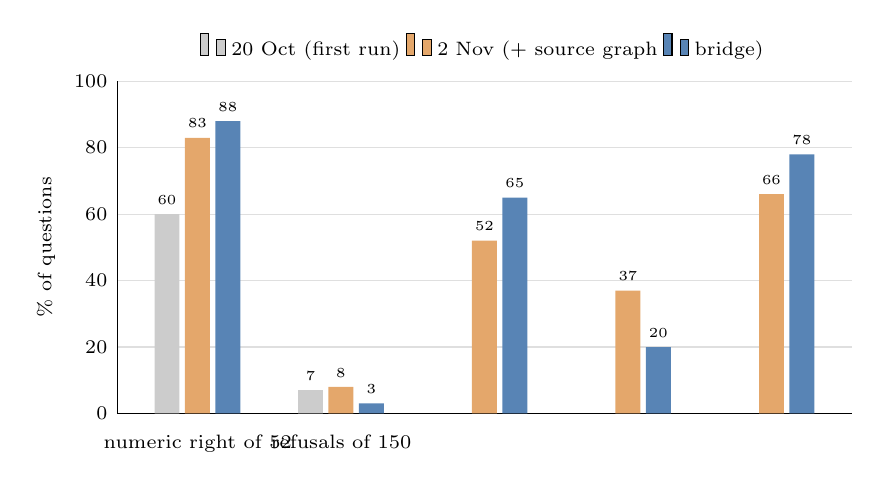
\begin{tikzpicture}
\begin{axis}[
  width=0.9\textwidth, height=58mm,
  ybar, bar width=9pt,
  ymin=0, ymax=100,
  ylabel={\% of questions},
  symbolic x coords={numeric right of 52, refusals of 150, text C of 98, text W+R of 98, overall of 150},
  xtick=data,
  x tick label style={font=\scriptsize,align=center,text width=24mm},
  y tick label style={font=\scriptsize},
  ylabel style={font=\scriptsize},
  legend style={font=\scriptsize,at={(0.5,1.03)},anchor=south,legend columns=3,draw=none},
  nodes near coords, nodes near coords style={font=\tiny},
  enlarge x limits=0.14,
  axis lines*=left, tick style={draw=none},
  ymajorgrids, grid style={gray!25},
]
\addplot[fill=gray!40,draw=none] coordinates {(numeric right of 52,60) (refusals of 150,7)};
\addplot[fill=cConnector!70,draw=none] coordinates {(numeric right of 52,83) (refusals of 150,8) (text C of 98,52) (text W+R of 98,37) (overall of 150,66)};
\addplot[fill=cEntity!85,draw=none] coordinates {(numeric right of 52,88) (refusals of 150,3) (text C of 98,65) (text W+R of 98,20) (overall of 150,78)};
\legend{20 Oct (first run), 2 Nov (+ source graph, bridge), 7 Nov (+ learned retriever)}
\end{axis}
\end{tikzpicture}
\caption{FinanceBench, the three full runs. Higher is better for the first, third and fifth groups; lower for refusals and wrong-or-refused text. Text grades were not recorded for the first run.}
\label{fig:fb}
\end{figure}


Between the first and second runs, 17 of the 21 numeric misses were traced to six causes and fixed in code (outflows printed in brackets used with their sign; a ratio returned $\times 100$ when no percent was asked; ``X as a \% of revenue'' kept as one target; a filer name not matching its legal form; a 10-Q's quarter read off the calendar month) and the source graph, the bridge and the re-read covers went in. Between the second and third, the learned retriever replaced the ladder. The finder's decisions did \emph{not} change in kind between those two runs (search again 42\% of reads, found 33\%, widen 18\%, absent 1\%); the better retrieval shows in the answers rather than in fewer re-searches.

\paragraph{What is still wrong, and why.}
The three numeric misses that are new in the last run are not retrieval. One identity was solved the wrong way round, so a derived net profit was recorded as a margin; one input was ``derived'' from 2 of a subtotal's 10 parts because the task cap stopped the search (the aggregation rule has no coverage floor, a gap known since September and the one thing the planned value rule replaces); and one question defined its ratio over \emph{average} inventory while the graph's identity uses ending inventory (a question's own definition must beat the graph's). The four refusals are a figure that sits in an 8-K's exhibit, a passage read but judged not to answer, and a quantity found in a note and in the cash-flow statement while the question asked for the income-statement line. Of the 17 wrong text answers, 6 are a verdict against the gold on a judgement call, 5 a wrong figure or sign, 4 a ``cannot determine'' where the gold has a value and 2 a figure not carried into the text. One text answer was given from the wrong company's filing, a document-choice error.

\paragraph{Against a published system.}
The one published system with per-question results on the same 150 questions is PageIndex (Mafin 2.5), a layout-tree index reasoned over by a model. Its authors report 136 of 150 answers ``aligned'' with the gold with rounding tolerated and 148 of 150 after adjudicating twelve golds as wrong or ambiguous. Set beside like, the 2 November run scores 97/150 (64.7\%) on the first ruler and 105/150 (70.0\%) under their rule applied by hand; the 7 November run's strict figure is 110/150 (73.3\%). The gap under any ruler is refusals (a refusal is wrong under every judge, and their run refuses nothing) and partial text answers (subsets of a list, which their superset rule does not accept). The one structural idea the two systems share, an index built from the document's own layout for a model to reason over rather than embeddings alone, is the part of their claim these results support; where this system differs is that every cited figure is checked in code against the printed cell, every derived value is recomputed from the graph's equation, and the formula is the graph's and not the model's.

\subsection{Cost}

Ingesting a filing costs two model calls and embeddings, about 30 seconds and \$0.15--0.30, with tables stored whole and never read by a model at ingest. Answering costs a median of 9 calls per question and 20 seconds; the whole 150-question run takes about two hours four questions at a time. Building the knowledge bases cost nothing at the model: the SEC relations were measured, the bridge counted, the retriever fitted on filings' own tags; the paid calls were the extraction of textbook equations (one per equation, in the first weeks) and the authoring and review agents of August and October.

\section{Limitations and the plan for the coming months}
\label{sec:next}

\subsection{What the results do and do not show}

The results show that a graph of verified equations, used as a prior over text that is read at question time with every citation checked, answers 88\% of the numeric FinanceBench questions and 78\% overall, that the graph's solver answers every textbook question once the naming is right, and that each of the pieces built this year (the source graph, the bridge, the learned retriever) produced a measured improvement when it went in. They do not yet show the claim at its strongest. FinanceBench questions name their company and period and mostly need one or two cells; the questions that the graph is \emph{for}, a quantity three equations away from anything printed, or a question over several filings, are under-represented in it, and the independent question set that the working agreements call for has not been written. Text answers are judged by reading, by me, against golds that are themselves sometimes arguable (FinanceBench's golds use three different quick-ratio formulas). And every comparison with another system is across different graders.

\subsection{Known defects}

\begin{itemize}
\item \textbf{Fixed caps instead of a value rule.} The loop stops on task, depth, route and round caps. Two misses in the last run came from a cap stopping a search that would have succeeded. The three numbers a proper stopping rule needs are now in hand: the calibrated bridge chance, the calibrated retrieval chance, and the reader's measured success rate.
\item \textbf{The aggregation rule has no coverage floor.} A total derived from 2 of 10 parts is reported with a note rather than refused.
\item \textbf{A question's own definition does not yet beat the graph's formula.} ``Inventory turnover over average inventory'' used the graph's ending-inventory identity.
\item \textbf{Graph quality.} Reviewers noted wrong bindings outside the repaired set, near-duplicate entities (``price change'' and ``lagged price change'' styles), and 75 groups of entities that share one pasted definition. A textbook equation mixes filing quantities with ones no filing prints (market price, required return), so a map alone unlocks an equation only when the rest is given or derived. The curated source corpus still writes \(E[\cdot]\); its loader was removed, so \code{finance\_sec.db} is now the only current form of the textbook graph.
\item \textbf{Bridge coverage.} The 20-F rows over-predict by half because the 2025 20-F filers tag IFRS while the bridge's rows are mostly US GAAP: the bridge needs a filer-class split. Only one quarter of the Notes data set is in; releases and 8-Ks have no tags and therefore no measured rows.
\item \textbf{Refusals.} A refusal is the design when no verified figure exists, and it is wrong under every benchmark grader. Four remain; each is a retrieval or reading failure, not an unanswerable question.
\item \textbf{Document choice} can still land on the wrong company's filing (one case), and one fourth of the finder's reads end in ``search again''.
\end{itemize}

\subsection{Plan}

\begin{enumerate}
\item \textbf{The value rule} (next): a worth per target passed down the formula tree, one queue of open actions ranked by worth $\times$ chance $\div$ cost, where chance is the calibrated bridge share times the calibrated retrieval mass times the reader's rate, with a floor replacing the caps. Then the coverage floor on aggregations and the question's definition taking precedence over the graph's.
\item \textbf{The independent question set}: questions written from real filings that need derivation through several equations, several documents (a 10-K and the following 10-Q, a parent and its co-registrant), and that the documents cannot answer, so that the method is measured on what it is for rather than on what the benchmarks happen to ask.
\item \textbf{DocFinQA on its test split}~\citep{reddy2024docfinqa} (922 questions, 240 filings; its questions are FinQA's~\citep{chen2021finqa} with the table removed, so they do not name their company, and only the test split was human-validated) and the FinanceBench run repeated after each change, both with every call logged.
\item \textbf{Graph repairs continued} by the same method as October: authored decisions applied by a refusing script, each exposed by a measurement or a reviewer; a filer-class split in the bridge; more Notes quarters.
\item \textbf{Writing up}: the entity--connector graph and its verification against filings; the commitment measurement and the graph-as-prior design; and the data arrangement for learned pieces (fit on filings that label themselves, evaluate on benchmarks whose companies never trained anything) as a methodological contribution of its own.
\end{enumerate}

The budget agreed for this project was that it should not delay the main thesis by more than six to eight weeks. It has grown beyond that because each measurement opened a tractable next step; the substrate it has produced (a verified equation graph over the SEC vocabulary, a graph of document kinds, and a measured bridge between them) is the one the thesis's reasoning layer was always going to need, and the loop of Section~\ref{sec:impl-loop} is a first instance of backward-chained reasoning over typed primitives with data dependencies, which is the thesis's subject.


{\footnotesize\setlength{\bibsep}{1.5pt}
\bibliographystyle{abbrvnat}
\bibliography{references}}

\end{document}
